\normalfont\normalsize
\chapter{Related Work}

Related work for task scheduling is generally found under ``task mapping'' or ``task allocation''. In recent times many articles discuss this topic,
as it is fundamentally different to actively researched topics that mark a certain resemblance, such as Task Scheduling in high performance 
computing systems. WSNs have unique requirements in respect to network lifetime, availability, reliability that make research previously done not 
applicable. The objective of these articles is to find schedules with balanced energy consumptions for tasks. These schedules will allow a higher
processing power of the resource-restricted WSN. Some research advocates splitting WSNs into lesser nodes and more powerful nodes, around which the other
nodes are gathered, cluster heads. The lesser nodes deal with lower level sensing tasks, while cluster heads deal with higher level processing tasks.
This generates an asymmetrical network that puts too much pressure on the cluster heads. Even if the cluster heads have much higher processing power and
are not energy restricted (they are connected to a power outlet), this deviates from the concept of a WSN as well as not being as applicable.
Hence the following related work is picked from those articles that either treat a WSN as homogenous, or as a heterogenous network in which there isn't
a lot of difference in processing power between types of nodes.

 Research that is covered here generally follows certain steps: 
\begin{itemize}
 \item Make general assumptions about how the network operates.
 \item Assume certain formulas to calculate chosen metrics.
 \item Schedule/allocate tasks.
 \item Simulate the network.
 \item Plot in relation to chosen performance metric, with the simulation data obtained.
 
\end{itemize}

\section{EcoMapS}
EcoMapS({\itshape \textbf{E}nergy-\textbf{co}nstrained Task \textbf{Map}pping and \textbf{S}cheduling}) is a scheduling system aimed to map and 
schedule tasks of an application with minimum schedule length subject to consumption constraints\cite{Yuan2007}. EcoMapS is application-independent, as it 
uses simple tasks with data dependencies noted in a Directed Acyclic Graph (DAG). 

The way EcoMapS considers that a WSN operates is based on a few assumptions:
\begin{itemize}
 \item The WSN for EcoMapS is considered to be formed from multiple clusters of homogeneous wireless networks.
 \item The algorithm is set to work in one of these clusters.
 \item Moreover, each of these clusters has a single-hop topology, each node can communicate with any other node in the cluster
directly.
 \item Each cluster executes the application that is setup beforehand, or sent over the air by base stations.
 \item Communication and processing withing the cluster head is scheduled by the cluster head.
 \item Time synchronization is believed to be available.
 \item Sensor nodes can process information and communicate wirelessly at the same time.
 \item Communications within a cluster do not overlap with communications in other clusters, due to different wireless channel.
\end{itemize}

\subsection{Application modelling}

%\begin{wrapfigure}[12]{r}{0.5\textwidth}
\begin{figure}
  \begin{center}
    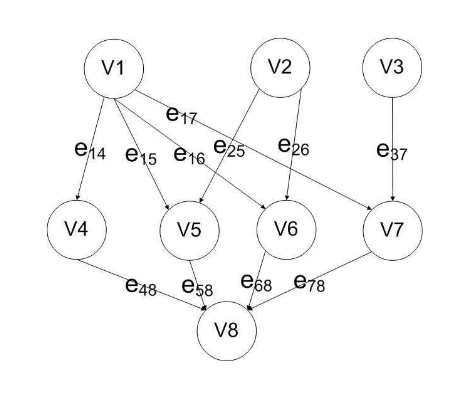
\includegraphics[width=60mm]{related/dag.png}
  \end{center}
  \caption{\small \itshape{ A task \textbf{D}irected \textbf{A}cyclical \textbf{G}raph}}
%\end{wrapfigure}
\end{figure}
Inter-dependence between tasks in the EcoMapS system is described with a DAG, which is a graph with directed edges where each edge
$e_{ij}$ means that task $v_j$ depends on task $v_i$, where  $v_i, v_j \epsilon V$, the set of tasks in the Directed Acyclic Graph.
The semantics associated with this graph is that a task $v_j$ cannot start execution until all its immediate predecessors (tasks 
$v_i$ where $e_{ij}$ is a directed edge in the graph) finish execution. Furthermore, the directed edge hints to the existence of 
data dependency between two tasks. If the two tasks adjacent to the edge are on the same node, execution for the second task can
begin immediately, otherwise it must wait for the transfer of results from the first task to complete before starting. This DAG 
is considered to have only one exit-task (a task with no successors), and as many entry-tasks (tasks with no predecessors) as needed.

The energy to transmit and to receive information wirelessly is given as a function of $l$, the number of bits, and $d$, the distance
between the two nodes that are communicated, $d$ being smaller than the largest distance of communication possible.
\begin{equation}
\label{energy1}
E_{tx} (l,d) = E_{elec} \cdot l + \varepsilon_{amp} \cdot l \cdot d^2
\end{equation}
\begin{equation}
E_{rx} (l) = E_{elec} \cdot l
\end{equation}
The energy consumption of executing $N$ clock cycles with clock frequency $f$ is considered to be:
\begin{equation}
E_{comp}(V_{dd},f) = NCV_{dd}^2 + V_{dd} (I_oe^{\frac{V_{dd}}{n V_T}})(\frac{N}{f})
\end{equation}


The problem to be solved is the mapping/scheduling of tasks, that is to find the set of assignments from task to node and the sequence
of execution that properly minimizes the objective function, which can be energy consumption or schedule length. Thus for each task 
($v_i$) we need an assigned node, $m_k$, with starting time $s_{i,m_k}$ and finish time $f_{i,m_k}$, execution length $t_{i,m_k}$ and
cost (representing energy consumption), $c_{i,m_k}$. An assignment is a tuple containing these value, 
$(v_i, m_k, s_{i,m_k}, t_{i,m_k}, f_{i,m_k}, c_{i,m_k})$, noted as $h_i$. Let $H^x = (h_1^x,h_2^x, ..., h_n^x)$, a schedule, with 
$x$ denoting the solution space. The result of the scheduling is to obtain $H^o \epsilon {H^x}$, a schedule which is optimal, meaning
it has minimum schedule length under energy consumption restraints. 

The problem is then formulated as: min $length(H^o)$, subject to $energy(H^o)$, where 
\[ length(H^o) = \max_{i,k} f_{i,m_k},\]
and
\[ energy(H^o) = \sum_{i,k} c_{i,m_k} \leq EB,\]
$EB$ being an ``Energy Budget''.

To model the communication channel in a cluster, the authors of EcoMapS use a virtual node $C$ that can execute communication tasks.
This is possible because at any given time, only one communication can take place, therefore the network topology can be converted from 
mesh to a star topology, where each node can communicate only with the center node $C$. Because communication costs are accounted for 
in the communication tasks themselves, cost to communicate from a normal node to $C$ is zero. Broadcasting is modelled as communication
from node to $C$, after which every node becomes a potential receiver.

%\begin{wrapfigure}[14]{r}{0.5\textwidth}
\begin{figure}
  \begin{center}
    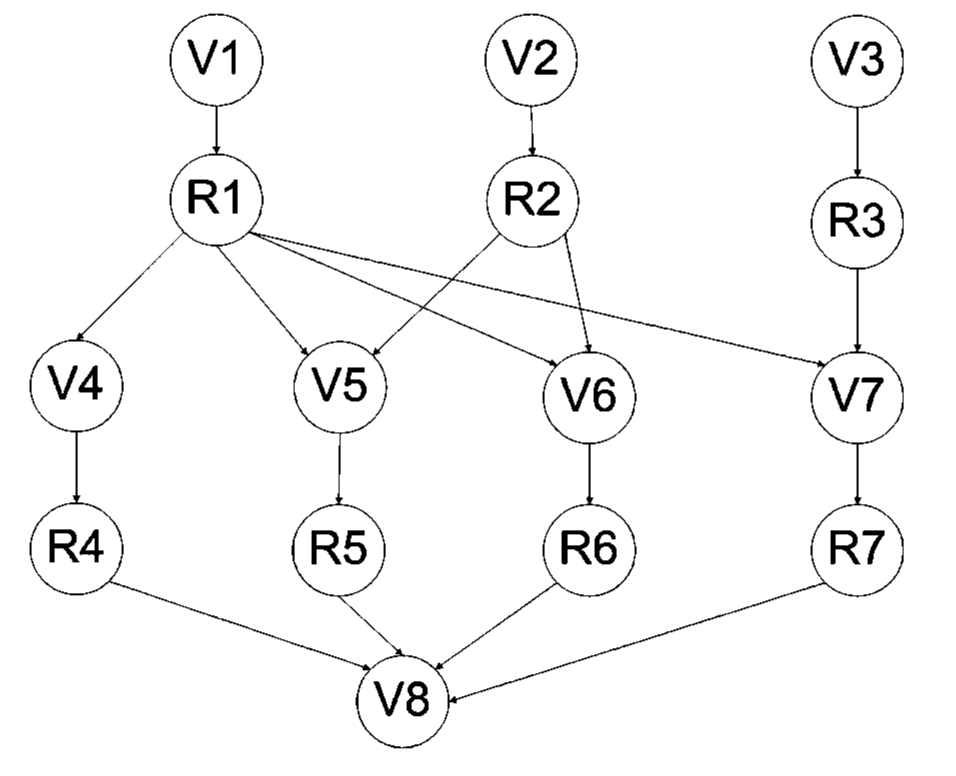
\includegraphics[width=60mm]{related/hyperdag.png}
  \end{center}
  \caption{\small \itshape{ A Hyper-DAG}}
%\end{wrapfigure}
\end{figure}
The next step is to include these communication tasks in the DAG. One way to do this is to add more nodes to the graph, nodes that
model communication tasks. Therefore, the new DAG, named Hyper-DAG, has a set of nodes $V' = V \cup R$, where $V$ is the set of computing
tasks and $R$ is the set of communicating tasks. Each processing task $v_i$ has only one successor, $R_i$, the communicating task
associated with delivering the results to tasks dependent on $v_i$. $R_i$ has all the successors there were previously attributed to
$v_i$. This new graph incorporates channel access conditions and broadcasting, along with the computing tasks.

The \textit{Dependency Constraint} is therefore reformulated for this type of DAG: \textit{If a computation task $v_j$ scheduled on node $m_k$
depends on a communication task $v_i$ on another node, a copy of $v_i$ needs to be scheduled to $m_k$, and $v_j$ cannot start to 
execute until all of its immediate predecessors are received on the same node.}

Scheduling communication in a single-hop network is done by duplicating the communication task from the sender node to $C$, then to each
of the receivers (in the case of a broadcast transmission). 

Because of the model adopted, in the process of task scheduling, several constraints have to be satisfied:
\begin{itemize}
\item A processing task cannot be assigned to the virtual node $C$,
{\large \[ \forall v_i \epsilon V, \; c_{v_i,C} = \infty, \: t_{v_i,C}=\infty. \]}
\item A communication task can be assigned both on processing nodes and on the virtual node.
\item If a communication task has its immediate predecessor and all of its immediate successors on the same node, it has no energy
cost or execution length (since no wireless communication needs to take place).
\item Other communication tasks have the energy estimation from formula \eqref{energy1}. 
\item If $v_i \, \epsilon \, V$ (computational task) and $\:pred(v_i) \neq \phi$, then 
\[ \:pred(v_i) \subset T(m(v_i))\,and\, s_{v_i,m(v_i)} \geq max f_{pred(v_i),m(v_i)} \]
\end{itemize}

\subsection{E-CNPT}
There are two phases described in the EcoMapS algorithm: The \textit{Initialization Phase} and the \textit{Quick Recovery Algorithm}, where
the former is a static scheduling of tasks involved in an application, whereas the latter is run when one of the nodes (not the cluster
head) fails. Constraints in place, the problem of initial scheduling is NP-complete, such that heuristic algorithms are needed to obtain
polynomial-time solutions. 


The \textit{Initialization Stage} follows somewhat the CNPT algorithm\cite{Hagr2005}, having two stages: \textit{listing stage} and 
\textit{sensor assignment stage}. The overall strategy is to assign the tasks along the most critical path to the nodes with the 
earliest execution start time (EEST).

The listing stage consists of sequentializing the tasks into a queue L such that the most critical
path comes first and each task is positioned after all its predecessors. First, the Earliest Execution Start Time is calculated for all
tasks. The entry-tasks have $EEST = 0$ and $EEST(v_i)$ is calculated by propagating the following formula through the Hyper-DAG downward,
from entry-tasks to exit-task:
\[ EEST(v_i) = \max_{v_m \epsilon pred(v_i)} \{EEST(v_m) + t_m, LST(v_i)\} \]

The Latest Execution Start Time can then be calculated following the Hyper-DAG in reverse direction, from exit-task to entry-tasks, starting
with the LEST = EEST for the exit-task and using the following formula:

\[ LEST(v_i) = \min_{v_m \epsilon succ(v_i)} \{LEST(v_m)\} - t_i \]

$t_i$ in this case is the execution time of a task $v_i\,\epsilon\,V$ on a sensor node or a task $v_i\,\epsilon\,R$ on $C$.

The next step of the listing stage is to push the tasks that represent Critical Nodes (tasks that have their $LEST(v_i)=EEST(v_i)$) on
a stack denoted as $S$. Following this, the top of the stack, $top(S)$ is investigated:
\begin{itemize}
\item If $top(S)$ has immediate predecessors that aren't on the stack or in the list, push the immediate predecessor with the minimum
LEST on the stack.
\item Otherwise, pop the stack and enqueue the popped task.
\end{itemize}

The listing phase ends when the stack is empty, the result is a list L with the order needed. In the next stage, the \textit{sensor
assignment stage}, task are dequeued from $L$ and assigned to the sensors with minimum execution time. The extended algorithm enhances 
this phase, running it several times for a different number of ``active'' nodes. If the schedule meets the deadline requirements, then
clearly it will consume less energy by using less nodes for the same application. The algorithm for one run is outlined in Listing \ref{cnpt},
the extension simply iterates over the number of nodes, choosing each time a set with one more ``active'' node.


\lstset{numbers=left, mathescape=true, title='SingleCNPT Algorithm', nolol=false,caption=Single CNPT Algorithm,label=cnpt}
\begin{lstlisting}
while L is not empty
  Dequeue $v_i$ from L
  if $v_i\,\epsilon\,R$ /* communication task */
    Assign $v_i$ to node $m(pred(v_i))$
  else if $pred(v_i) = \phi$ /* entry-tasks */
    Assign $v_i$ to node $m_i^o$ with min $EAT(m_i^o)$
  else /* non-entry computation tasks */
    for all computing sensors $\{m_k\}$
      Calculate $EST(v_i,m_k)$:
      if $pred(v_i)\,\subseteq\,T(m_k)$
        $EST(v_i,m_k) \leftarrow max(EAT(m_k), f_{pred(v_i),m_k})$
      else /* communication is needed */
        for $v_n\,\epsilon\,pred(v_i) - T(m_k)$
          $CommTaskSchedule(v_n,m(v_n),m_k)$
        $EST(v_i,m_k) \leftarrow max(EAT(m_k), f_{pred(v_i),m_k})$
  Keep the schedule with $min(EST(v_i,m^o))$
  Schedule $v_i$ on $m^o$:$s_{v_i,m^o} \leftarrow EST(v_i,m^o)$
\end{lstlisting}



\begin{itemize}
\item $T(m_k)$ denotes the tasks assigned on node $m_k$.
\item $m(v_i)$ denotes the node on which $v_i$ is assigned.
\item $pred(v_i)$ and $succ(v_i)$ are the immediate predecessors/successors of task $v_i$.
\item $EAT(m_k)$ is the Earliest Available Time on node $m_k$.
 ×
\end{itemize}

The idea is simple: we assign communication tasks to the node where the data-generating task (for that communication, that is to say the immediate predecessor
in the Hyper-DAG) was assigned. If the task is an entry-task, we assign it to the node with the earliest available time. If it is a non-entry computing task,
we check if we're generating the earliest execution time for the same node, and if we are, mark it as the ending of the predecessor task (in the Hyper-DAG), or
the earliest available time on that node (whichever is later). If it isn't the same node, then we need communication: we propagate the communication task to the 
virtual node and to the recipients. Once the propagation is done, we can once more see when the task can be schedulet earliest. We then schedule the task on the node
that appeared to have the earliest time of all. 


\subsection{E-MinMin}

A second algorithm developed for the Initialization Phase of EcoMapS is also based on a simpler algorithm, MinMin, and searches for the optimal number of computing 
sensors that has the smallest schedule length with an energy constraint. For each assignment $(v,m)$, MinMin algorithm calculates a \textit{fitness} function $fit(v,m,\alpha)$.
The fitness function expresses the cost in time and energy of assigning task $v$ to node $m$. $\alpha$ is a trade-off parameter that weighs in for time or for energy.


\lstset{numbers=left, mathescape=true, title='SingleMinMin Algorithm', nolol=false,caption=Single MinMin Algorithm,label=minmin}
\begin{lstlisting}
for $\alpha = 0;\,\alpha\leq1.0;\, \alpha+=\delta\alpha$
  for entry-tasks $v_i$
    Assign $v_i$ on node $m_i^o$ with $min\:EAT(m_i^o)$
    Assign $succ(v_i)$ on $m_i^o$
  Initialize the mappable task list $L$
  while $L$ is not empty
    for task $v_i\,\epsilon\,V$
      for all computing nodes $m_k$
        if $pred(v_i)\nsubseteq T(m_k)$
          for $v_n\,\epsilon\,pred(v_i)-T(m_k)$
            $CommTaskSchedule(v_n,m(v_n),m_k)$ 
	    /* propagate communication task */
        Calculate $fit(v_i,m_k,\alpha)$
      Find $m_i^o:\:fit(v_i,m_i^o,\alpha)=min$
    Find $(v,m):\: fit(v,m,\alpha) = min$
    Assign $v$ to $m$, remove $v$ from $L$
    Assign $succ(v)$ on $m$
    Update $L$ with unassigned mappable tasks
Among schedules with different $\alpha$
  if $\exists H\,:\,energy(H) \leq EB$
    Return $H^o:\:length(H) = min$
  else 
    Return $H:\:energy(H) = min$
\end{lstlisting}


The main idea behind Listing \ref{minmin} is to map computational tasks, leaving communication tasks on the same node, leaving them to propagate with the
function $CommTaskSchedule( , , )$. Among all possible assignments, the one that is most fit is chosen at each step.

\subsection{Quick Recovery Algorithm}

As previously mentioned, WSN have special requirements for scheduling algorithms. Node failure is common in WSNs, so one such requirement is for the algorithm 
to have failure handling. As rescheduling from scratch is not efficient, EcoMapS proposes a quick recovery solution: assign the tasks of the failed sensor to the 
sensor with the most idle time.

\subsection{Outcome}

EcoMapS aims to minimize schedule lengths of applications under energy consumption constraints. Using the channel model and communication scheduling
algorithm, EcoMapS simultaneously schedules communication and computation tasks. Simulation show that EcoMapS is quite performant in respect to other similar 
algorithms. E-MinMin based EcoMapS outperforms the other version, although E-CNPT-based EcoMapS has less computing overhead. The former would then be best 
suited for stable networks, while the other would be for WSNs where updates are more frequent.

\section{Real-time support in Wireless Sensor Networks}

A different aspect of the scheduling problem is scheduling a given set of tasks (can be repeteable) on a single node, taking into account energy efficiency, as done
in \cite{Deli2005}. For the scheduler to be able to make correct, power-aware decisions, tasks that are set to execute on the node must specify a worst 
execution time and a deadline, as well as an indicator of ``importance''. This ``importance'', also denoted as a power index, shows the relative importance 
of a task in relation to the other tasks under low-power conditions. 

%\begin{wrapfigure}[10]{r}{0.5\textwidth}
\begin{figure}
  \begin{center}
  \vspace{-20pt}
    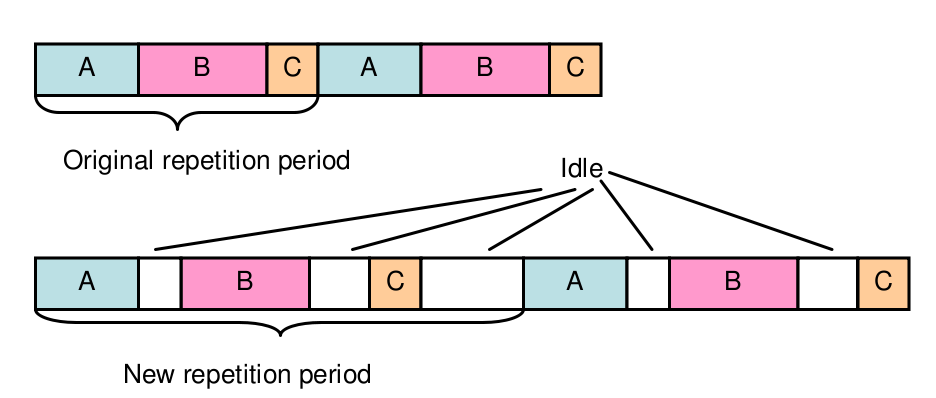
\includegraphics[width=80mm]{related/idle.png}
  \end{center}
  \caption{\small \itshape{Idle time insertion through deadline extension}}
%\end{wrapfigure}
\end{figure}

The main idea is that to extend network lifetime, non-critical tasks will be scheduled at greater intervals. All tasks have an initial deadline; if the sensor node
is in a low-energy state (~30\% battery left), then the tasks runs a piece of code to redetermine its deadline in respect to the remaining battery life. 
Extending the deadlines for most of the tasks executing on the node can mean that there's time left in which the MCU is idle, which is supposed to consume
less power than in the active state, hence the average power consumption is lowered and network lifetime increases.

\subsection{PA-EDF}

Power-Aware Earliest Deadline First is a scheduling algorithm based on EDF that can make power-aware decisions when dequeueing tasks. If the battery level is above
a certain threshold, tasks are scheduled in the same way as in EDF. Once the battery level drops below a threshold, tasks with the power-index smaller than the 
threshold are considered ``important'' and are scheduled in the same way, while tasks with larger power-index are given a chance to reconsider their power-index,
reducing the frequency with which they execute at the same time.

\subsection{APA-EDF}

Adaptive Power-Aware Earliest Deadline First is similar to PA-EDF, the difference being that there is more than one threshold, there are $n$ thresholds, where $n$
is also the number of power indexes possible. Each power index is associated with a threshold. Each time the scheduler dequeues a task, it checks its power index
against the current battery remaining and acts accordingly, either it schedules it or executes the special reanalysis code.  

\subsection{Findings}

PA-EDF and APA-EDF successfully incorporate the power consumption issue into realtime scheduling, increasing the network lifetime overall by increasing the lifetime
on each of the nodes. These algorithms allow the network to focus on the more important tasks, reducing the frequency of less important tasks when batteries are low.


    
\section{The SENSEI project}

SENSEI (Integrating the Physical with the Digital World of the Network of the Future) is a project integrated in EU's 7th Framework Programme for Research
an Technological Development.

\begin{figure}[h]
 \begin{center}
  
\includegraphics[scale=0.25]{wsan/sensei.png}
 \end{center}

\end{figure}


SENSEI is meant to help build the network of the future, integrating Wireless Sensor and Actuator Networks (WS\&ANs) into a framework of global scale. This 
framework is envisioned as service oriented, because WSANs are by nature heterogeneous. WSAN islands should be able to offer services through a unified service
interface to be integrated more easily in different applications. Network and information management services will ensure correct functioning of these islands
and proper adjustment to the ever-changing physical environment. Accounting, security, privacy and trust are also key issues in integrating these islands in the
network of the future.


Goals of the SENSEI project are:
\begin{itemize}
\item \textbf{Scalability of the framework} - The protocols that are part of the framework must support easy integration of very many WS\&AN islands 
into a global network. New networks must have plug and play integration into the greater network, allowing for greater ease of use of WS\&ANs. 
\item \textbf{An open service interface} - Unification of application access to information and actuation services. This will help the development of new
applications onto already connected/existent WS\&AN networks
\item \textbf{Efficient WS\&AN island solutions} - Aim of this being wireless transmission with 5nJ/bit, by using energy-aware protocol stacks, and ultra low-power
transceivers. This would greatly increase network lifetime of a WS\&AN network.
\item \textbf{Pan European test platform} - A large scale experimentation and field trials of proposed technologies, evaluating the progress of integration
of WS\&ANs into the Future Internet.
\end{itemize}


\section{Applications of Wireless Sensor Networks}
\subsection{Industrial Control and Monitoring}

Wireless sensor networks can be used in industrial environment with a great deal of success. Usually an industrial
facility consists of a small control room and the rest of the physical plant. This control room has indicators and displays
from different sensors throughout the plant, as well as inputs for actuators. Instead of using expensive thick cables to
connect the control room to the sensors and actuators, a wireless sensor network can be used.

The conditions for this type of network would be that reliability has to be high, conditions that can be satisified by a network
with many nodes and many possible routing paths from each node to the data sink (positioned or connected to equipment in the control
room).

Possible applications here are in industrial safety, for instance, a network that detects presence of noxious, poisonous or
dangerous materials on a plant. Significant notice needs to be given to WSNs with self-healing and self-maintenance,
which will be resilient enough to be able to gather data in the event of an explosion/damage on the plant.

Another use of WSNs would be in monitoring or control of rotating/moving heavy machinery, reducing the possibility of
accidents due to collisions. A wired solution would be undesirable for this application, for instance in the case of a rotating
piece of equipment wires would hinder its freedom of movement. 

Present HVAC systems (Heating, Ventilation and Air Conditioning) suffer from lack of data, they generally have a few
thermostats per building. The end result is a large difference in air temperature in the building between different rooms. A wireless sensor
network would be able to cover a lot more space, gathering enough information for the system to be truly efficient. A smart HVAC system,
with the help of an appropriate sensor system, would know that activities in one room keep it hot, while activities in another room (or
positioning in relation to cardinal directions) keep it cool, and would be able to correctly decide how to circulate air between them,
keeping them cool in summer and warm in winter.

\subsection{Home Automation}

Wireless sensor networks are particularly useful in homes, where adding wires is not always easy. A WS\&AN inside the home could communicate 
with a ``universal'' remote control (for electronic devices, curtains, locks, etc. ). Another concept that is related to home automation is 
Remote Keyless Entry (RKE), either for the home itself or for the car. 

Monitoring room temperatures can be applied in home automation as well, wireless temperature monitoring can be a good replacement for a 
normal thermostat, and would not need any extra wiring. The heating system could then maintain the same temperature throughout the house,
room by room. It could also discover room where insulation needs to be upgraded. Rather than upgrade insulation for the entire home, which
is costly, the owner could then upgrade only the insulation responsible for the heat loss. Wireless sensor networks make intelligent home 
monitoring systems more accesible and more powerful.

\subsection{Security/Military Sensing}

WSNs can act as sentries around defensive perimeters, or can be used to identify and locate targets on a battlefield. They are easy to deploy on
the battlefield and can be well hidden (camouphlaged as rock, mounds or what-not), are robust because there is no single point of failure (with
multiple alternate routing paths), making them difficult to destroy in battle.

Target tracking is a good example of a collaborative application of WSNs. Sensor nodes must take measurements then process them distributively
to find the location of moving targets or classify targets.
\subsection{Asset Tracking and Supply Chain Management}

An example of asset tracking with WSNs would be an intelligent warehouse, where each object can be easily found because it has a node with an id. This
boosts the efficiency of the warehouse, because a lost object can be a lost sale, while taking the same costs by occupying space in the warehouse.
Management of large objects can indeed be aided by the use of a WSN, as with railroad cars in railyards, or shipping containers in a port. Managing
containers is a lot more sensitive since the containers are stacked onto one another, and removing a container at the bottom is a costly operation. Having
precise information about the location of each container needed makes way for the use of an algorithm such that the entire process can be optimized.
\subsection{Intelligent Agriculture and Environmental Sensing}

A common known fact is that water is a major factor for plant growth. While too little water means reduced yields, too much leads to drainage and
diseases. Thus a very important part of agriculture is water-management. What WSNs give is the ability to make localised decisions instead of global ones.
Field conditions are not uniform, and treating the problem as if they were means that some portions of the field might be under-irrigated, while others
might suffer from excessive application. Wireless rain gauges and humidity sensors could monitor the status of the field, as well as control individual 
sprinklers in a zone. This leads to a system that is water-efficient, energy-efficient, low-cost and autonomous, as demonstrated in \cite{Yuns2007}. 
Use of WSNs can be extended to use of chemical and biological sensors to asses the need for pesticides, herbicides and fertilizers, or to search for 
contaminants such as mercury. 

As for Environmental sensing, the main use is for early detection of natural disasters such as floods, earthquakes or forest fires, as well as monitoring 
grand scale fenomena, i.e. glacier movement. A WSN to detect forest fire could be deployed by releasing the nodes from a helicopter, 
thus reaching in remote places. Nodes would have to be self-sufficient or have enough network lifetime to be worth using. WSN nodes with 
temperature and humidity sensors could be clustered in the forest around a special gateway node that could communicate the data with a 
mobile network access technology (e.g. UMTS). 

WSNs can help minimize damage produced by an earthquake by assessing the structural integrity of a building. Nodes would be scattered along the walls and in
critical spots and they would measure structural responses to external vibrations, inferring the structural integrity. 

\subsection{Health monitoring}

WSNs is  starting to invade the non-life-critical health monitoring. This means athletic performance monitoring, 
an athlete carrying a BSN (Body Sensor Network) will execute his exercise then he will be able to assess both his 
performance and his body's response to the effort. Professional and semi-professional athletes have already been using these
wireless network to monitor pace, heart rate and distance, but the technology should start covering recreational athletes as well. 

Inside the hospital WSNs could form a night watch assistance system, were non-life-critical parameters such as temperature could 
be monitored on a set of pacients, reducing the need for the nurse to check their health status constantly.

Real medical applications will be slow in emerging, due to regulations and very high need for robustness and accuracy.


